\section{Entity relationship diagram}
\subsection{Description}

\begin{flushleft}
Afin de sauvegarder, modifier et supprimer des données, il est nécessaire d'implémenter la notion de factures dans la base de données. C'est pourquoi, ce diagram illustre l'ajout de factures.
\end{flushleft}

\begin{flushleft}
Tout d'abord, une facture est liée à un contrat. C'est pourquoi, nous retrouvons une liaison entre un contrat et une facture. En outre, un élement "id_factures" a été ajouté à l'entité "contrat" afin de relier les 2.\footnote{"id_factures" étant un Primary Key}
\end{flushleft}

\begin{flushleft}
Ensuite, l'entité "factures" regroupe plusieurs variables : 
\end{flushleft}
\begin{enumerate}[-]

\item \textbf{"id_contrat" relie la facture au contrat avec un varchar de 10 caractères.}

\item \textbf{"statut" contient une valeur binaire du statut de paiement.}

\item \textbf{"ideal_accompte" contient une valeur double de l'accompte proposé par l'application.}

\item \textbf{"methode_paiement" contient une valeur binaire du mode de paiement.}

\item \textbf{"paiement_informations" contient un varchar avec les informations bancaires du client.}

\end{enumerate}

\begin{figure}[h]
\subsection{Schéma}
\centering
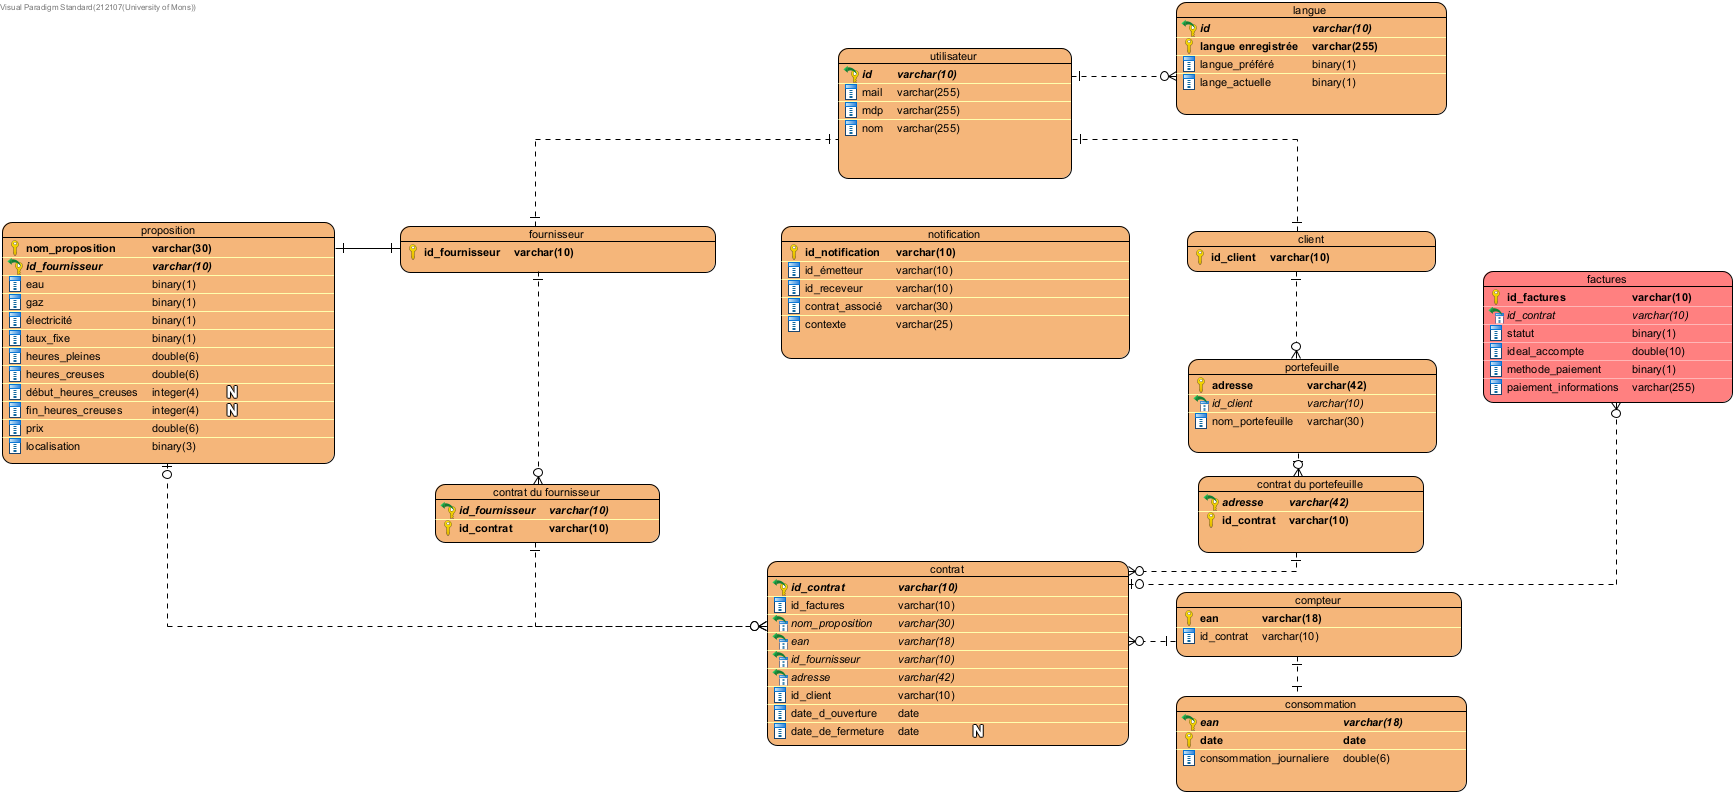
\includegraphics[width = 1]{extension-maxime/bdd/bdd-extension.png}
\end{figure}
